\section{Selection status of every component}
\label{sec:supp_selection}
Table~\ref{tab:supp_status} lists how each component of the final pipeline entered it. Two components were adopted after the registered rule kept a simpler reference; their registered outcomes are reported here in full.

\begin{table*}[t]
\centering
\footnotesize\setlength{\tabcolsep}{4pt}
\begin{tabular}{@{}>{\raggedright\arraybackslash}p{5.2cm}l>{\raggedright\arraybackslash}p{9.0cm}@{}}
\toprule
Component & How it entered & Registered evidence \\
\midrule
CA without 32-px modules & promoted & 4/5 folds, OOF 0.665$\rightarrow$0.691, paired CI $[+0.015,+0.029]$ \\
All CA heads and calls, conditional query, mean of word pieces & promoted / kept & head and call subsets inside the 0.002 tie band once crossed with scale \\
SA module 15 (64 px) & promoted & 5/5 folds, 0.756$\rightarrow$0.789 \\
Two observation-wise passes & promoted & 0.788$\rightarrow$0.800; confirmed with DenseCRF in 5/5 folds (0.813) \\
DenseCRF, fixed parameters & promoted & 5/5 folds, all 20 classes improved in its screen \\
SA calls 10--20 & promoted & selected after DenseCRF in 4/5 folds (selection path 0.8158 vs.\ 0.8132) \\
SA-guided layer weights & \textbf{owner decision} & forced 4/5 folds, +0.0061 OOF, COCO +0.018; multi-candidate screen chose it in 3/5 folds and kept uniform \\
Coarse-to-fine hierarchy with one-sided cap & \textbf{owner decision} & forced 5/5 folds vs.\ fine-only and plain hierarchy; selectors kept fine-only because the worst class lost 0.057--0.104 in the training folds (guard: 0.050); training-fold gain +0.0039 to +0.0071 \\
\bottomrule
\end{tabular}
\caption{\textbf{Selection status.} ``Owner decision'' marks components adopted after the pre-registered selector retained its reference. Their numbers in the main paper are forced out-of-fold estimates, never in-sample, and their COCO-Cap numbers are frozen transfer.}
\label{tab:supp_status}
\end{table*}

\paragraph{The negative record at a glance.}
Figure~\ref{fig:supp_decision_map} places the 45 registered comparisons of the fine-only phase (studies up to SG28) against the reference of its own run; Sec.~\ref{sec:supp_packages} lists them, and Sec.~\ref{sec:supp_record} gives every cell.

\begin{figure*}[t]
\centering
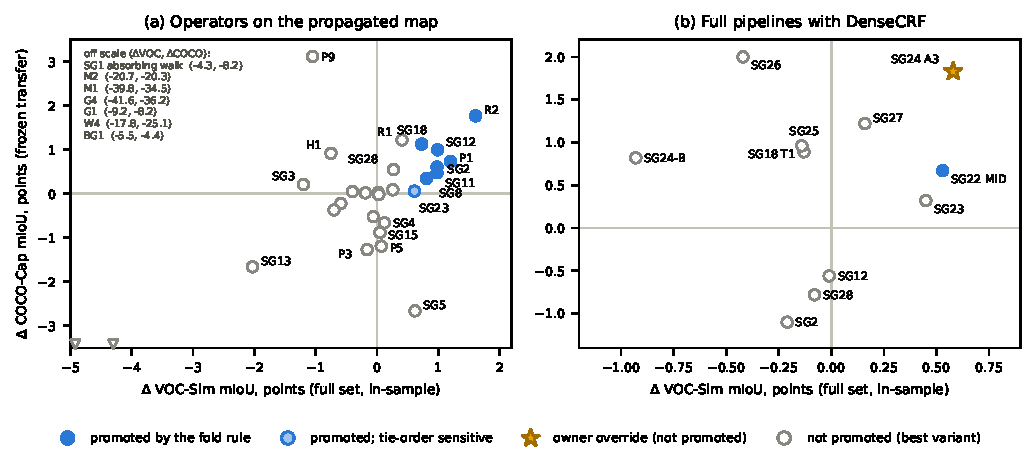
\includegraphics[width=\textwidth]{figures/decision_map.pdf}
\caption{\textbf{The search at a glance.} Each point is one registered experiment family, compared with the reference cell of the same run. $x$: change in VOC-Sim mIoU at each cell's full-VOC threshold (in-sample, descriptive); $y$: change in frozen COCO-Cap transfer. (a) Operators on the propagated map, mostly against one SA pass. The promoted cluster (blue) gains about one point on both datasets, but apart from the second pass and DenseCRF these operators do not improve on two passes plus DenseCRF. (b) Complete pipelines with DenseCRF. Only the middle-call window is promoted, and the SA-guided weighting (star) was adopted by owner decision. Several multi-scale studies raise COCO-Cap transfer but are not selected on VOC-Sim. The map covers the studies up to SG28; later studies, including the hierarchy, are in Secs.~\ref{sec:supp_stages} and \ref{sec:supp_record}.}
\label{fig:supp_decision_map}
\end{figure*}
\clearpage
